\documentclass{beamer}

%Colorir Ruby
\usepackage{minted}

% Codificação UTF-8
\usepackage[brazilian]{babel}
\usepackage[utf8]{inputenc}

% Imagens
\usepackage{graphicx}

% Tabela
\usepackage{xcolor,colortbl}
\definecolor{gray}{rgb}{0.87,0.87,0.87}

\usetheme{CambridgeUS}


\clearpage

\title{Banco de Dados e Relacionamento}


\subtitle{Rais - Dia 4}

\author[Felipe e Akme-re]{~Felipe Fernandes \and ~Akme-re Almeida}

\institute[Fabsoft] % (optional, but mostly needed)
{}

\date{}

\AtBeginSubsection[]
{
  \begin{frame}<beamer>{Outline}
    \tableofcontents[currentsection,currentsubsection]
  \end{frame}
}

% Let's get started
\begin{document}

\begin{frame}

  \titlepage
  
\end{frame}

\begin{frame}{Agenda}
  	\tableofcontents
  % You might wish to add the option [pausesections]
\end{frame}
\begin{frame}[fragile]

\frametitle{Banco de Dados - Conceito}
\section{Banco de Dados}
%\subsection{Conceito}
\begin{block}{\LARGE Conceito}
	\begin{itemize}
		\item \LARGE Coleção de dados armazenados em uma maquina.
		\item \LARGE Base que pode ser acessada por softwares para consultas e atualizações.
	\end{itemize}
\end{block}

%\begin{minted}[linenos,xleftmargin=50]{rb}
%  	def lol
%  		 "hello world"
%  	end
%  	
%  	:sym
%  \end{minted}
\end{frame}

\subsection{First Subsection}

\begin{frame}[fragile]{Banco de Dados}{Exemplos}
	\begin{columns}
		\begin{column}{0.5\textwidth}
			\begin{figure}
				\begin{minipage}{\columnwidth}
					
\includegraphics[scale=0.5]{images/pg}
				\end{minipage}
				\begin{minipage}{\columnwidth}
					
\includegraphics[scale=1]{images/mysql}
				\end{minipage}
			\end{figure}
		\end{column}
	
		\begin{column}{0.5\textwidth}
			\begin{figure}
				\begin{minipage}{\columnwidth}
					
\includegraphics[scale=0.7]{images/oracle}
				\end{minipage}
				\begin{minipage}{\columnwidth}
					
\includegraphics[scale=0.5]{images/sqlite}
				\end{minipage}
			\end{figure}
		\end{column}
	\end{columns}		
\end{frame}


\begin{frame}[fragile]{Ferramenta}{SQLiteman - Ferramenta gráfica para gerenciar o Banco}
	\begin{figure}
		\begin{minipage}{\columnwidth}
			\centering
				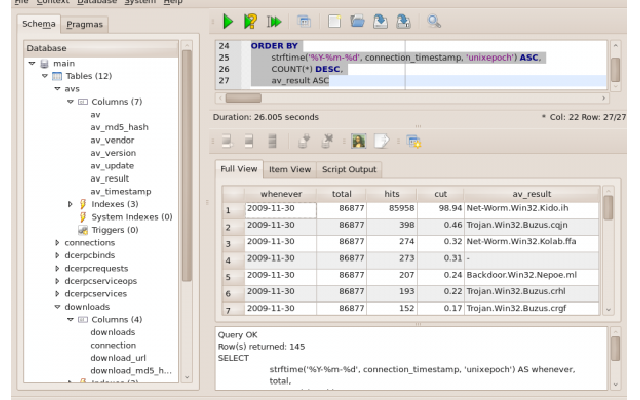
\includegraphics[scale=0.4]{images/sqliteman}
		\end{minipage}
	\end{figure}
\end{frame}
%\subsection{Second Subsection}

% You can reveal the parts of a slide one at a time
% with the \pause command:
\begin{frame}[fragile]{SQLite 3}{Default Rails}
	\begin{itemize}  \itemsep 2em
		\item{ \LARGE Banco de Dados Simples.}
		\item{ \LARGE Apenas para Estudo.}
		\item{ \LARGE Não deve ser usado em projetos robustos.}
		\item{ \LARGE Banco de dados localizado em um unico arquivo.}
								
	\end{itemize}
\end{frame}
%\section{Second Main Section}

%\subsection{Another Subsection}

\begin{frame}{Banco de Dados}{Conceitos Iniciais}
	\begin{itemize} 
		\item{
			\LARGE Bancos Possuem o que?
			\begin{itemize} \itemsep 2em
				\item{ \Large Usuários - Autenticação}
				\item{ \Large Schemas - Organização}
				\item{ \Large Tabelas - Armazenamento}
			\end{itemize}
		}
	\end{itemize}
\end{frame}

\begin{frame}{SQLite}{Tabela}
	\begin{itemize} 
		\item{
			\LARGE Tabelas
			\begin{itemize} \itemsep 2em
				\item{ \Large Estruturas de armazenamento para os dados.}
				\item{ \Large Schemas - Organização.}
				\item{ \Large Tabelas - Armazenamento.}
			\end{itemize}
		}
	\end{itemize}
\end{frame}
% Placing a * after \section means it will not show in the
% outline or table of contents.
%\section*{Summary}

\begin{frame}{Tabela}
	\begin{center}
		\begin{table}
			\LARGE
			\caption{\label{label}\Large Dividas.}
			\begin{tabular}{ c | l }
					\hline
					\hline
					\hline					
					\cellcolor{gray} \textbf{CONTA}  & \cellcolor{gray}\textbf{VALOR} \\
					\hline
					Luz & 100.50 \\
					\hline
					Agua & 50.55 \\
					\hline
					Telefone & 45.50 \\
					\hline
					\hline
			\end{tabular}% Tabulação
		\end{table}
	\end{center}
\end{frame}



% All of the following is optional and typically not needed. 
\appendix
\section<presentation>*{\appendixname}
\subsection<presentation>*{For Further Reading}

\begin{frame}{Index e Chave Primária}
	\begin{center}
		\begin{table}
			\LARGE
			\caption{\label{label}\Large Dividas.}
			\begin{tabular}{ c | l | c}
					\hline
					\hline
					\hline					
					\cellcolor{gray} \textbf{ID} & \cellcolor{gray} \textbf{CONTA}  & \cellcolor{gray}\textbf{VALOR} \\
					\hline
					1 & Luz & 100.50 \\
					\hline
					2 & Agua & 50.55 \\
					\hline
					3 & Telefone & 45.50 \\
					\hline
					\hline
			\end{tabular}% Tabulação
		\end{table}
	\end{center}
\end{frame}

\begin{frame}{Chave Estrangeira}
	\begin{block}{\LARGE Chave Estrangeira - Conceito}
		\begin{itemize}
			\item \LARGE Index Especial que liga duas Tabelas para melhor aproveitamento
		\end{itemize}
	\end{block}
\end{frame}

\begin{frame}{Relacionamentos}{Tipos}
	\begin{itemize} \itemsep 2em
		\item{ \LARGE 1 x 1 }
		\item{ \LARGE 1 x N }
		\item{ \LARGE N x N }
	\end{itemize}
\end{frame}

\begin{frame}{Cardinalidade}{1 e 1}
	\begin{center}
		\begin{table}
			\Large
			\caption{\label{label}\Large Pessoas.}
			\begin{tabular}{ c | l | c}
				\hline
				\hline
				\hline					
				\cellcolor{gray} \textbf{ID} & \cellcolor{gray} \textbf{NOME}  & \cellcolor{gray}\textbf{NASCIMENTO} \\
				\hline
				1 & Rodrigo Andrade Leal & 01/09/1994 \\
				\hline
				2 & Felipe Almeida Zamora & 05/10/1990 \\
				\hline
				\hline
			\end{tabular}% Tabulação
		\end{table}
	\end{center}
		
	\begin{center}
		\begin{table}
			\Large
			\caption{\label{label}\Large Documentos.}
			\begin{tabular}{ l | l | l | l }
				\hline
				\hline
				\hline					
				\cellcolor{gray} \textbf{ID} & \cellcolor{gray} \textbf{IDENTIDADE}  & \cellcolor{gray}\textbf{CPF} & \cellcolor{gray}\textbf{PES-ID} \\
				\hline
				55 & 55997-65  & 555.999.777 & 2\\ 
				\hline
				56 &  56587-65 & 544.455.545 & 1\\
				\hline
				\hline
			\end{tabular}% Tabulação
		\end{table}				
	\end{center}

\end{frame}

\begin{frame}{Cardinalidade}{1 e 1}
	\begin{center}
		\begin{table}
			\Large
			\caption{\label{label}\Large Pessoas.}
			\begin{tabular}{ l | l | l | l}
				\hline
				\hline
				\hline					
				\cellcolor{gray} \textbf{ID} & \cellcolor{gray} \textbf{NOME}  & \cellcolor{gray}\textbf{NASCIMENTO} & \cellcolor{gray}\textbf{DOC-ID} \\
				\hline
				1 & Rodrigo Andrade Leal & 01/09/1994 & 56\\
				\hline
				2 & Felipe Almeida Zamora & 05/10/1990 & 55\\
				\hline
				\hline
			\end{tabular}% Tabulação
		\end{table}
	\end{center}
		
	\begin{center}
		\begin{table}
			\Large
			\caption{\label{label}\Large Documentos.}
			\begin{tabular}{ l | l | l }
				\hline
				\hline
				\hline					
				\cellcolor{gray} \textbf{ID} & \cellcolor{gray} \textbf{IDENTIDADE}  & \cellcolor{gray}\textbf{CPF} \\
				\hline
				55 & 55997-65  & 555.999.777\\ 
				\hline
				56 &  56587-65 & 544.455.545\\
				\hline
				\hline
			\end{tabular}% Tabulação
		\end{table}				
	\end{center}

\end{frame}

\begin{frame}[allowframebreaks]
  \frametitle<presentation>{For Further Reading}
    
  \begin{thebibliography}{10}
    
  \beamertemplatebookbibitems
  % Start with overview books.

  \bibitem{Author1990}
    A.~Author.
    \newblock {\em Handbook of Everything}.
    \newblock Some Press, 1990.
 
    
  \beamertemplatearticlebibitems
  % Followed by interesting articles. Keep the list short. 

  \bibitem{Someone2000}
    S.~Someone.
    \newblock On this and that.
    \newblock {\em Journal of This and That}, 2(1):50--100,
    2000.
  \end{thebibliography}
\end{frame}

\end{document}


